\documentclass[11pt]{report}
\usepackage{geometry, graphicx, kotex, imakeidx, titlesec, array} % necessary packages
\usepackage{mathptmx}   
\usepackage{amsmath, amsthm, amssymb, mathrsfs, multirow, verbatim} % supplementary packages
\usepackage[nobiblatex]{xurl} % enable linebreak of \url command
\usepackage{indentfirst} % force indentation at every first paragraph of chapters, sections and subsections
\usepackage{booktabs} % table tool
\usepackage{ragged2e}
\usepackage{setspace}
\usepackage{natbib}
%%%\usepackage[style=apa,backend=biber]{biblatex}
%%%\addbibresource{references.bib}

\geometry{letterpaper, left=38mm, right=25mm, top=25mm, bottom=25mm}  % set the paper size and the margins
  
\titleformat{\chapter}{\normalfont\LARGE\bfseries}{\chaptertitlename\ \thechapter.}{20pt}{\LARGE} % chapter style
\newtheorem{theorem}{Theorem} % theorem environment
\newtheorem{definition}{Definition} % definition environment
% if you need similar environments like lemma, corollary or remark, add them all.
\makeindex % command for making an index chapter

\linespread{1.5} % set the vertical spacing between successive lines (the ratio of the maximal height of a normal font and the base lineskip)

\renewcommand\arraystretch{1.3} % increase the vertical spacing by 30%

%%% stands for a new chapter or a new page
%% stands for a new section
% stands for a comment

%%%%
%\input{macros}

\begin{document}

\newpage 
\begin{center}
\huge Testing a Modern Inference Framework for POMP Models: A Case Study Using Stochastic Volatility  
\par\vspace{1cm} % spacing can be adjusted
\begin{figure}[ht]
\begin{center}

\includegraphics[width=.4\textwidth]{umichlogo.png}
\end{center}
\end{figure}
{\fontsize{16pt}{16pt}\selectfont by \par Dae Hyun Kim \par} % put the student's name here
\vspace{1.0cm}
\par\vspace{0.2cm}
{\fontsize{16pt}{18pt}\selectfont Supervisor Professor: Edward Ionides \par} 
\vspace{0.7cm}
\vspace{10pt}
{\fontsize{16pt}{16pt}\selectfont Department of Statistics \par }  % You can reduce the character spacing to make the department name on one line. If it takes up more than two lines, please reduce the vertical spacing after the title appropriately.
\vspace{1.5cm}
{\fontsize{18pt}{18pt} University of Michigan\par} 
\vspace{1cm}
{\fontsize{14pt}{14pt}\selectfont April 2025}
\end{center}

\newpage 
\pagenumbering{roman} % set the page number as roman type from this page on.
\newgeometry{left=30mm, right=30mm, top=30mm, bottom=30mm} % set the paper size and the margins
% Margins shall be changed to bottom and top 3 cm, right and left 2 cm from this page forward.
\addcontentsline{toc}{chapter}{Abstract}
\begin{center}
\par\vspace{20pt}
\large \textbf{Abstract}
\end{center}

\normalsize
\justifying % this command available with \usepackage{ragged2e}
\doublespacing
The pypomp package is a new Python-based library for modeling likelihood-based inference on partially observed Markov process (POMP) models. Designed with the same goals as the R package pomp, pypomp offers a flexible environment for modeling nonlinear, non-Gaussian dynamic systems and supports both standard particle filtering and gradient-based estimation methods. By leveraging modern computational tools such as automatic differentiation (AD) and GPU acceleration via JAX, pypomp enables efficient inference for POMP models. We test and validate the pypomp package by using the Heston stochastic volatility model as a test case. Through this case study, we indicate the potential of pypomp to serve as a robust, extensible tool for scientific modeling and the development of advanced inference algorithms.
\par

\par\vspace{20pt}
\textbf{Keywords}: iterated filtering, automatic differentiation, stochastic volatility

\newpage


%%% table of contents
\renewcommand*\contentsname{Table of Contents}
\addcontentsline{toc}{chapter}{Table of Contents}
\tableofcontents

\bigskip


%%% first chapter of the main body

\chapter{Introduction}\label{chap:intro}
\pagenumbering{arabic} % set the page number as Arabic type from this page on.
Inference for dynamic systems governed by latent processes is a core process in modern statistical science, with applications to various fields such as epidemiology, ecology, and finance. Partially observed Markov process (POMP) models, also known as hidden Markov models or state space models provide a principled framework for modeling such systems, in which a latent stochastic process drives an observed time series. However, only partial and noisy observations of the true underlying state are available in POMP models and general Maximum Likelihood Estimate (MLE) is often infeasible due to the intractability of the likelihood, which involves integrating over high-dimensional latent state spaces. 


The improved Iterated Filtering (IF2) algorithm introduced by \textbf{\citet{ionides2015inference}}, suggests an alternative to approach these challenges. IF2 uses the particle filter, also known as sequential Monte Carlo (SMC) method, to estimate parameters in POMP models and it iteratively refines parameter estimates by introducing stochastic perturbations to the parameters, which facilitates convergence to the MLE. IF2 is a plug-and-play method that enables parameter estimation without requiring analytic expressions for transition densities, making it applicable to a wide variety of scientific models such as epidemiology 
\textbf{\citet{subramanian2021quantifying}}, \textbf{\citet{wheeler2024informing}}, \textbf{\citet{king2008inapparent}}(numerical results from \textbf{\citet{ionides2015inference}}), ecology \textbf{\citet{li2024inference}}, and finance \textbf{\citet{szczepocki2020application}}, \textbf{\citet{sunmodel}}.


The R package pomp has provided a powerful framework including IF2 for likelihood-based inference on POMP models \textbf{\citet{king2016statistical}}, but with the growing use of Python in scientific computing, there is a need for a library with similar modeling capabilities that also support modern numerical frameworks. In response to these needs, the pypomp package is being developed as a Python-based analog to pomp, and it supports plug-and-play particle filtering and simulation for POMP models, but it is also designed as a library for new algorithmic development. Key innovations in pypomp include the use of automatic differentiation (AD) for efficient gradient computation and the integration of JAX for just-in-time (JIT) compilation and GPU acceleration, enabling significant computational efficiency. One of the central algorithmic contributions of pypomp is the Iterated Filtering with Automatic Differentiation (IFAD) algorithm, introduced by \textbf{\citet{tan2024accelerated}}. Unlike IF2, which relies on stochastic perturbations for optimization, IFAD integrates gradient based updates through AD. This approach improves computational efficiency by combining rapid exploration of the parameter space via stochastic perturbations with precise gradient refinement. The use of AD also enables us to take advantage of just-in-time compilation, making IFAD particularly suitable for large scale data. However, as pypomp is currently at early stages of development, it requires rigorous testing to ensure its correctness, stability, and reproducibility across applications.


We verify the operations of pypomp by using the Heston stochastic volatility model as a diagnostic benchmark. \textbf{\citet{sunmodel}} applied the IF2 algorithm using the pomp package in R to estimate the parameters of the Heston stochastic volatility model and we attempted to replicate these results using IF2 in pypomp. We then apply IFAD within the pypomp framework to estimate the same model parameters, comparing the inference quality, stability, and computational efficiency. Rather than focusing on improved inference for the Heston model itself, this research uses the model as a structured test case for evaluating the behavior and correctness of the pypomp. Our numerical results indicate both the promise and current limitations of pypomp, providing insights into its potential as a library for scientific inference and methodological research in dynamic systems.


%%%  the second chapter of the main body
\chapter{Background}\label{chap:background}

\section{Iterated Filtering Algorithms}
The key idea behind IF2 is to embed the estimation of parameters within a particle filter by introducing small random perturbations to the parameters across time steps. These perturbations are gradually reduced over multiple iterations, enabling the algorithm to stochastically explore the likelihood surface and converge toward the MLE. Unlike its predecessor, IF1 introduced by \textbf{\citet{ionides2011iterated}}, which approximates the score function via conditional moments, IF2 performs an iterated Bayes map, providing more robust numerical properties and convergence guarantees. (pseudocode in Appendix A)

The particle filter is a foundational tool for inference in POMP models. It enables likelihood-based \textbf{\citet{ionides2006inference}} and Bayesian inference \textbf{\citet{chopin2013smc2}}, \textbf{\citet{andrieu2010particle}} by providing Monte Carlo estimates of the likelihood function of observed data given model parameters. Specifically, the particle filter approximates the likelihood by simulating a collection of possible latent trajectories(particles) and sequentially weighting them according to how well they explain the observed data. This approach is both flexible and powerful, particularly for models where the latent dynamics are nonlinear and non-Gaussian \textbf{\citet{arulampalam2002tutorial}}, \textbf{\citet{kitagawa1987non}}. On top of that, the particle filter produces an unbiased estimate of the likelihood \textbf{\citet{doucet2001sequential}}, making it suitable for likelihood-based inference as it only requires accurate estimates for the likelihood. As a result, IF2 builds directly on the particle filter to perform plug-and-play likelihood maximization


The advantages of IF2 are its plug-and-play flexibility and stochastic robustness. Specifically, IF2 does not require the evaluation of transition densities, which allows it to be applied to models defined via simulation and the iterative perturbation process helps avoid early convergence to the local optima, which is common in complex likelihood surfaces. Also, the numerical results from \textbf{\citet{ionides2015inference}} indicate that IF2 can approximate the MLE arbitrarily well, under mild regularity conditions, as the number of particles and iterations increase.


The original implementation of IF2 was developed in the R package pomp, but R presents limitations in computational scalability, especially for models requiring GPU acceleration or AD. This is where Python and the pypomp become critically useful. The field of Python research has grown rapidly due to its integration with high-performance libraries like JAX, as well as GPU-accelerated frameworks. As pypomp leverages modern features such as JIT compilation and AD, it makes it particularly well-suited for research using large-scale data.




\newpage
\section{Automatic Differentiation Particle Filter}
Automatic Differentiation (AD) is a computational process that enables the efficient and accurate calculation of derivatives for functions implemented as computer programs. Also, AD computes exact derivatives by systematically applying the chain rule to a sequence of elementary operations \textbf{\citet{rall1996introduction}}, \textbf{\citet{verma2000introduction}}. This capability is particularly powerful in fields such as machine learning, numerical optimization, and scientific computing, where gradient based methods are used.

AD operates by breaking down a function into a finite sequence of elementary operations and computing their derivatives step-by-step. AD can be implemented in two primary modes:
\begin{enumerate}
    \item \textbf{Forward Mode}:
    \begin{itemize}
        \item Computes derivatives by propagating derivatives from the inputs to the outputs.
        \item Efficient for functions with few inputs and many outputs.
    \end{itemize}
    \item \textbf{Reverse Mode}:
    \begin{itemize}
        \item Computes derivatives by propagating gradients backwards from the outputs to the inputs.
        \item Efficient for functions with many inputs and few outputs.
    \end{itemize}
\end{enumerate}
Both modes rely on the chain rule to propagate derivatives through computation:
\[\frac{\partial f}{\partial x} = \frac{\partial f}{\partial y} \cdot \frac{\partial y}{\partial x}\]

Recent work has extended the use of AD to particle filtering and inference for POMP models. The advantage of using AD is the gradient-based optimization for POMP models. Several research have explored differentiable particle filters. For instance, \textbf{\citet{jonschkowski2018differentiable}} introduced differentiable filtering networks, and \textbf{\citet{naesseth2018variational}} proposed variational inference approaches using AD to optimize latent state models. However, these early approaches typically relied on low variance but asymptotically biased estimators of the gradient, raising concerns about their long-term reliability and statistical guarantees.

The Automatic Differentiation Particle Filter (ADPF), introduced by \textbf{\citet{tandifferentiable}}, overcomes these issues by framing the particle filter as a differentiable computational graph. On top of that, \textbf{\citet{tan2024accelerated}} introduces Measurement Off-Parameter with discount factor $\alpha$ (MOP-$\alpha$) algorithm that defines estimators for the gradient of the log-likelihood where the estimators balance the tradeoff between bias and variance. At $\alpha = 0$, low-variance estimators can be highly biased, while at $\alpha = 1$, unbiased estimators tend to suffer from high Monte Carlo variability. MOP($\alpha$) interpolates between these extremes, allowing users to refine the factor based on precision needs.

The Iterated Filtering with Automatic Differentiation (IFAD) algorithm introduced by \textbf{\citet{tan2024accelerated}} represents another development of using ADPF. IFAD algorithm incorporates MOP-based gradient estimators into the structure of the IF2 algorithm. Like IF2, IFAD executes a stochastic perturbation of parameters through a particle filter. However, instead of fully relying on perturbations to update parameter estimates, IFAD supplements this process with gradient-based updates using AD. This process enables IFAD to overcome the two core challenges of IF2 such as Monte Carlo variability from noisy perturbation updates and slow convergence in high-dimensional spaces.

\newpage
\section{Stochastic Volatility Models}
Stochastic volatility models play a central role in financial modeling, where accurately capturing the evolution of asset price variability is crucial for derivative pricing, risk management, and portfolio allocation. Among these models, the Heston model is widely used due to its ability to represent volatility as a mean-reverting stochastic process. However, parameter estimation for such models is challenging because of the intractability of their likelihood functions and the presence of latent variables.

The estimation of parameters in stochastic volatility models remains a challenging problem, primarily due to the computational complexity of the likelihood function, which involves high dimensional integration. Various methods have been developed to address these challenges. \textbf{\citet{ait2007maximum}} developed a maximum likelihood estimation method that addresses these challenges by employing closed-form approximations to the likelihood function. \textbf{\citet{chib2002markov}} and \textbf{\citet{chib2006analysis}} developed Markov Chain Monte Carlo (MCMC) algorithms for generalized stochastic volatility models. However, these methods are computationally intensive for high dimensions.

%Volatility is a measure of the variability or uncertainty of asset prices, and it is a fundamental concept in finance. The modeling of volatility is crucial for applications such as option pricing and risk management. Traditional models, such as the Black-Scholes model from \textbf{\citet{black1973pricing}, assume constant volatility over time. However, the evidence from financial markets such as volatility smile \textbf{\citet{derman1994riding} has shown that volatility is not constant but varies over time and traditional models often fail to reflect real-world dynamics. This has implied the development of stochastic volatility models and volatility started to get regarded as a stochastic process. 

The Heston model introduced by \textbf{\citet{heston1993closed}}, one of the most widely used stochastic volatility models includes a mean-reverting stochastic process for volatility, revealing the limitations of constant volatility models. Specifically, it assumes that the variance of asset returns follows a Cox-Ingersoll-Ross (CIR) process, expressed as:
\[d\nu_t = \kappa(\theta - \nu_t) \, dt + \xi \sqrt{\nu_t} \,dW_t^\nu\]
where 
\begin{itemize}
    \item $\nu_t$ is the instantaneous variance of the asset price at time $t$,
    \item $\kappa$ is the rate of mean reversion in variance, 
    \item $\theta$ is the long-term mean level of variance ($\lim_{t \to \infty} \mathbb{E}[\nu_t] = \theta$),
    \item $\xi$ is the volatility of the volatility,
    \item $W_t^\nu$ is the Wiener process in the volatility,
\end{itemize}
Simultaneously, the asset price $S_t$ changes according to the following stochastic differential equation:
 \[dS_t = \mu S_t\, dt + \sqrt{\nu_t} S_t \, dW_t^S\] 
 where:
\begin{itemize}
\item $S_t$ is the asset price at time $t$,
\item $\mu$ is the average growth rate of the asset price 
\item $W_t^S$ is the Wiener process in the asset price
\end{itemize}
 
The Heston model provides a realistic framework for understanding how volatility changes over time, enabling more accurate pricing of financial instruments and better investment decisions with market uncertainty. Therefore, it is effective for testing and comparing parameter estimation algorithms, such as the IF2 algorithm and the IFAD algorithm.
\newpage



\chapter{Iterative Filtering in pypomp}\label{chap:organizing}
\textbf{\citet{sunmodel}} applied the IF2 algorithm implemented in the R package pomp to estimate the parameters of the Heston stochastic volatility model using daily S$\&$P500 log-return data from 2010 to 2024. His study indicated the ability of IF2 to recover volatility dynamics consistent with market benchmarks like the VIX index, and showed the model significantly outperformed classical GARCH-based benchmarks in terms of log-likelihood. His research also conducted profile likelihood estimation on each parameter, initially profiling over $\mu$, and subsequently fixing $\mu$ at its smoothed profile MLE to improve optimization stability. In our study, we sought to replicate Sun’s results using the pypomp package. While Sun performed profiling to construct confidence intervals, we did not require profiling of $\mu$ in our setting since our goal was not to conduct inference but to test and validate the numerical behavior of the pypomp IF2 implementation. 
%%

%%
\section{Log-likelihood Trace}\label{sec:ll_trace}
The log-likelihood trace records the IF2 log-likelihood estimate at each iteration. It is computed using perturbed parameters and is noisy, but the trend should generally increase (or negative log-likelihood should decrease). This is an internal measure during optimization progress, and it indicates whether the IF2 is improving the model fit during iterative process.

To evaluate the internal optimization process of both pomp and pypomp, we compared the log-likelihood values estimated at each iteration of the IF2 algorithm.
\newpage
%\bigskip
\begin{figure}[ht] 
\begin{center}
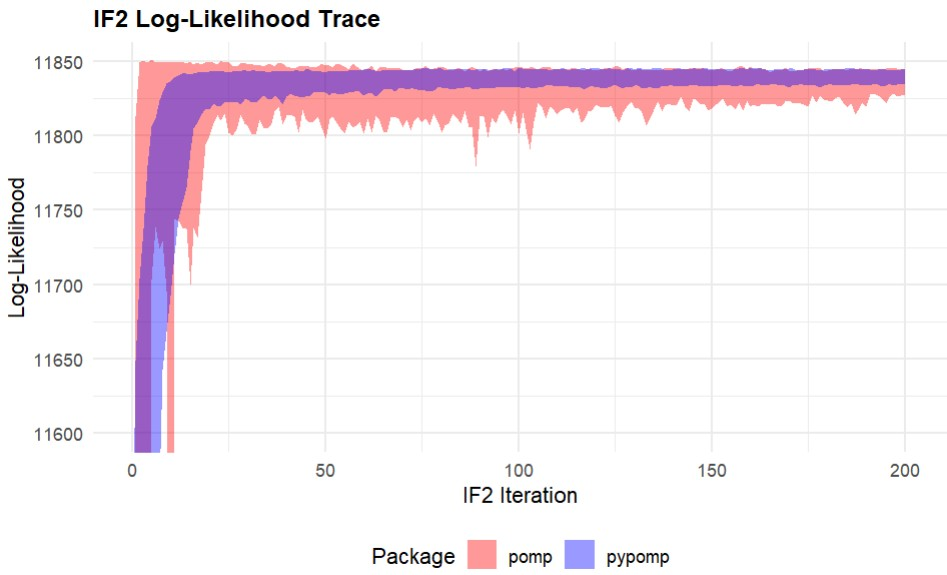
\includegraphics[width=\textwidth]{lltrace_zoomed.jpg}
\end{center}
\caption{IF2 Log-likelihood Traces across Iterations (Outliers excluded)}
\label{fig:if2lltrace}
\end{figure}
Each shaded ribbon in Figure 3.1 represents the 10th–90th percentile range of log-likelihood values across 120 IF2 replicates at each iteration. The values are computed using perturbed parameters during IF2 and represent noisy estimates of model fit throughout optimization. Although stochastic, the log-likelihood trajectories are expected to improve across iterations as the algorithm converges toward high-likelihood regions.
The results show that similar convergence behavior in both implementations, with pypomp exhibiting slightly more stable optimization dynamics. This indicates that not only the IF2 algorithm is functioning properly in both packages, but also there are differences between IF2 in pomp and IF2 in pypomp.



%%
\section{Parameter Estimate Trace}\label{sec:param_est}
The parameter estimation traces show the evolution of each parameter across IF2 iterations. We average across particles at each iteration to visualize the path of optimization. As parameters are iteratively perturbed and adapted toward the MLE, parameter estimation traces are important in the IF2 process. With this trace, it is available to analyze whether parameter estimates converge or diverge and whether they exhibit similar dynamics in pomp and pypomp. Also, if both implementations use the same algorithmic parameter values, cooling fraction, random walk standard deviation and starting points, their traces should be similar. This implies that parameter estimation traces provide qualitative assurance between pomp and pypomp.


To assess the consistency of the pomp implementation and pypomp implementation, we compared the evolution of parameter estimations across IF2 iterations. 


\begin{figure}[ht]
\begin{center}
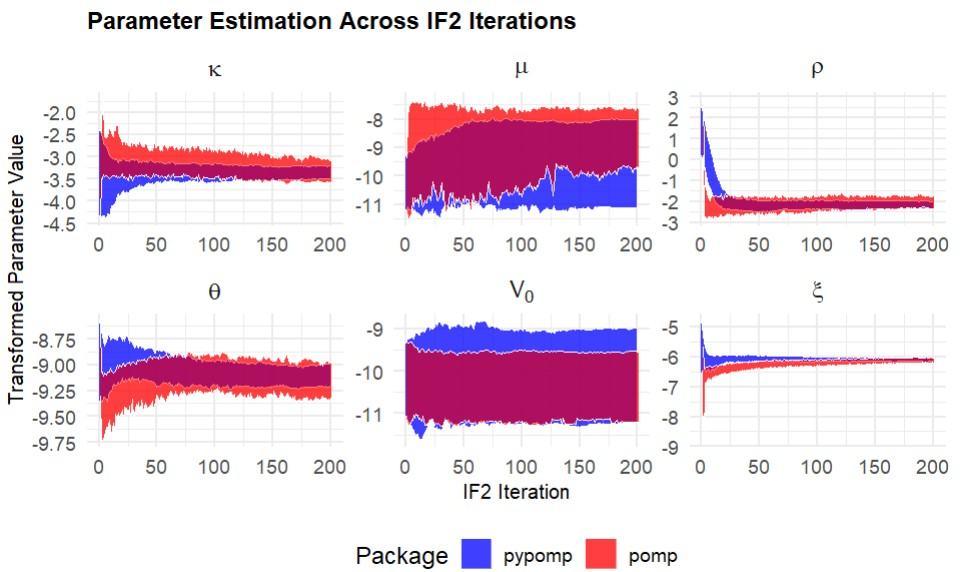
\includegraphics[width=\textwidth]{param_trace.jpg}
\end{center}
\caption{Parameter Estimation Across IF2 Iteration}
\label{fig:if2paramtrace}
\end{figure}


Figure {3.1} displays quantile ribbon plots showing the evolution of parameter estimates over IF2 iterations across pomp and pypomp implementations. For each parameter, we show the middle 80\% (10th to 90th percentile) of transformed parameter values at each iteration.
The parameters are transformed to the estimation scale such as log-transformed for positive parameters ($\mu$, $\kappa$, $\theta$, $\xi$, $V_0$) and logit-transformed for the correlation parameter ($\rho$). This transformation ensures a reasonable comparison since both implementations optimize in transformed space. 

Across all six parameters, we observe similar convergence behavior between the two implementations. Both implementations stabilize similarly to transformed values, indicating agreement in the inferred parameter regions but still there are noticeable differences in the median trajectories. 

Then, we assess whether the two implementations arrive at consistent parameter estimate.
\begin{figure}[ht]
\begin{center}
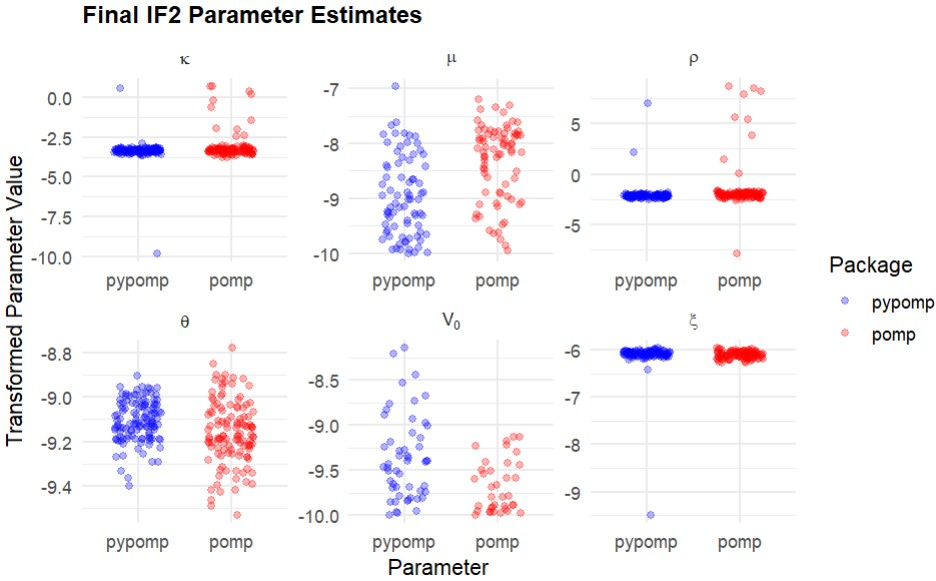
\includegraphics[width=\textwidth]{param_final.jpg}
\end{center}
\caption{Parameter Estimation at Final IF2 Iteration}
\label{fig:if2paramtrace2}
\end{figure}

Figure 3.3 displays the transformed parameter estimates at the final IF2 iteration from 120 independent IF2 runs in both pomp and pypomp. Each point represents the final parameter estimate from one IF2 replicate, transformed to the estimation scale (log or logit).
Across parameters, the distributions of final estimates are similarly aligned between the two implementations. Slight differences in spread and central tendency appear in $\mu$ and $V_0$ and these results indicate that while the two implementations do not produce identical traces, they broadly agree in terms of convergence region and variability. 

\section{Particle Filter Log-likelihood}\label{sec:pfilter}
After IF2 finishes, the algorithm uses a particle filter with particles and no perturbation to estimate the log-likelihood at the final estimated parameters. For each IF2 run, the algorithm computes the average and standard deviation of estimated log-likelihoods over particle filter replicates. The average log-likelihood assesses the fit quality of the estimated parameters, and the standard deviation gives a sense of Monte Carlo variability.
With these results, given the same number of particles and datasets, IF2 algorithm in both pomp and pypomp yield likelihood estimates with similar accuracy and variability.

To compare the model fit quality across implementations, we examined the log-likelihood values obtained by applying a particle filter to the final parameter estimates from each IF2 run. 
\begin{figure}[ht] 
\begin{center}
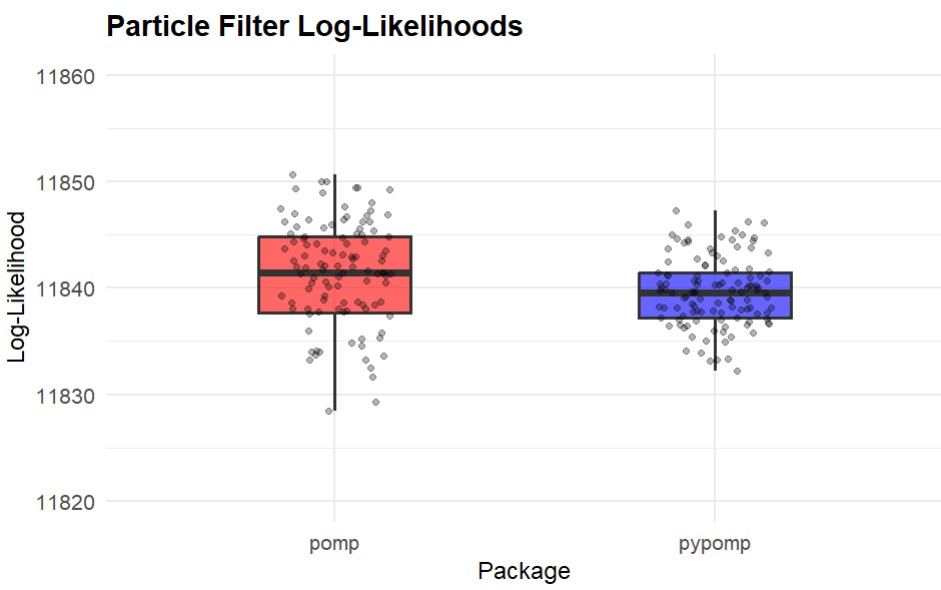
\includegraphics[width=\textwidth]{boxplot_zoomed.jpg}
\end{center}
\caption{Particle Filter Log-likelihood at Final IF2 Estimates(Outliers excluded)}
\label{fig:pfilterplot}
\end{figure}

Figure 3.4 shows a comparison of the log-likelihoods from particle filter evaluations at final IF2 estimates across 120 replicates. Each point represents the mean log-likelihood across iterations for one IF2 replicate. While pomp shows a slightly higher median and broader spread with 11850.74 for the highest log-likelihood, pypomp shows lower median and tighter spread with 11847.34 for the highest log-likelihood.

To verify that particle filter in pypomp matches the behavior of the pomp, we conducted a Monte Carlo-based comparison. Using the same stochastic volatility model and the MLE for each parameter obtained from pomp, we evaluated the log-likelihood using standard particle filter without parameter perturbation across 24 replicates in pypomp. The best log-likelihood estimated with the MLE in pomp was 11850.74 and the best log-likelihood estimated with the MLE in pypomp was 11848.29 with standard deviation 2.78. These results support the conclusion that the particle filter in pypomp reproduces the behavior of pomp up to expected Monte Carlo variation and the discrepancy between pypomp and pomp stems from IF2 perturbation. 

\newpage
\chapter{ADPF in pypomp}\label{chap:adpf}
\textbf{\citet{tan2024accelerated}} demonstrate that IFAD outperforms both IF2 and MOP algorithms when applied individually. IF2 alone is prone to slow convergence near the optimum due to diminishing perturbation sizes and MOP alone is sensitive to local minima and saddle points in non-convex likelihood surfaces. The strengths of IFAD are a warm start using IF2 to locate a neighborhood near the MLE and a refinement that uses gradients derived from the MOP-α estimator to perform gradient ascent with AD. This hybrid approach helps IFAD to overcome two critical limitations of IF2 and MOP.

Using the cholera transmission model that developed for Dhaka, Bangladesh \textbf{\citet{king2008inapparent}}, IFAD found log-likelihood values significantly better than those reported using IF2 \textbf{\citet{ionides2015inference}}. Notably, IFAD reaches the MLE with fewer iterations and without the assistance of likelihood profiling. These results indicate IFAD's numerical efficiency and statistical accuracy, and its potential as an innovative plug-and-play method for statistical inference in POMP models.

Encouraged by the numerical efficiency and statistical accuracy of IFAD, we attempted to analyze its performance implemented in pypomp using the Heston stochastic volatility model from \textbf{\citet{sunmodel}}. However, during the implementation and testing of IFAD and MOP in pypomp, we encountered persistent numerical instabilities such as NaNs and exploding values. Despite initializing the algorithm with plausible parameter values and a reasonable number of particles, NaN gradients and log-likelihood values frequently occurred during the optimization after the first forward mode of AD, suggesting issues within the backward mode of AD execution. As these instabilities do not occur in IF2 implementation of pypomp, it reinforces the conclusion that the source of instability comes from the gradient refinement in MOP implemented in pypomp. 


%%% the third chapter of the main body
\chapter{Conclusion}\label{chap:conclusion}
Our research contributes to the development, testing, and validation of the pypomp package. Using the Heston stochastic volatility model as a test case, we examined the behavior and correctness of the IF2 and IFAD algorithms in pypomp, comparing results against pomp package.
For IF2, we demonstrated that pypomp implementation successfully produces log-likelihood estimates and parameter traces that are consistent with the general behavior of IF2. However, despite these promising results, a discrepancy remains between the IF2 results from pypomp and those from pomp, particularly in log-likelihood and parameter estimation across iterations. Based on diagnostic comparisons, we conclude that these differences are unlikely to come from the particle filter but rather from the IF2 perturbation process.
For IFAD, although the algorithm is theoretically well-supported and has shown success in recent research, we encountered persistent numerical instabilities when attempting to apply IFAD to the Heston model in pypomp. These issues include NaN gradients and log-likelihood values, and failures in the optimization after the initial iteration. These findings indicate that while IFAD is a prominent method, the current pypomp implementation requires further refinement, particularly in how gradients are calculated and handled within the JAX AD system.


\chapter{Discussion}\label{chap:discussion}
This research reveals two main directions for improving the robustness and reliability of inference in pypomp.
\section{Improving IF2 Compatibility and Correctness}
Although the particle filter in pypomp appears to behave as expected, full equivalence with pomp's IF2 implementation will require deeper examination of the IF2 update procedure. Specifically, how JAX’s JIT compilation interacts with random number generation and parameter perturbation logic should be investigated and the reproducibility should be ensured by managing PRNG keys explicitly in all stochastic components. 
\section{Stabilizing and Benchmarking IFAD}
The numerical instability observed when applying IFAD in pypomp suggests issues in how gradients are computed and propagated, particularly through resampling and parameter update steps. Future development should ensure differentiability of the computational graph across all IFAD components and manage numerical stability in weight scaling and normalization, especially in the MOP-$\alpha$ gradient estimators. Beyond debugging, IFAD must be evaluated through performance benchmark tests that measure runtime efficiency, memory usage, and number of iterations required to reach convergence. These tests are particularly important for assessing IFAD's scalability and practical utility for statistical inference.


\newpage


\renewcommand \bibname{Reference}
\addcontentsline{toc}{chapter}{Reference}
%%%\printbibliography
\bibliographystyle{plainnat}
\bibliography{references}
%make citet -> \textcite
\vspace{1cm}
\normalsize



%%% the appendix chapters
\newpage
\appendix
\addcontentsline{toc}{chapter}{Appendix}
\chapter{Algorithms}
\noindent\textbf{Algorithm 1 IF2} \\[0.5em]
\noindent\textbf{Algorithm 2 MOP-$\alpha$} \\[0.5em]
\noindent\textbf{Algorithm 3 IFAD} \\[0.5em]

\begin{tabular}{@{}p{0.98\textwidth}@{}}
\textbf{Input:} Number of particles $J$, timesteps $N$, measurement model $f_{Y_n|X_n}(y_n^*|x_n, \theta)$, simulator process $f_n(x_{n+1}|x_n, \theta)$, evaluation parameter $\theta$, behavior parameter $\phi$, seed $\omega$. \\[0.5em]

\textbf{First pass:} Set $\theta = \phi$ and fix $\omega$, yielding $X_{n,j}^{P,\phi}, X_{n,j}^{F,\phi}, g_{n,j}^\phi$. \\

\textbf{Second pass:} Fix $\omega$, and filter at $\theta \neq \phi$. \\

\textbf{Initialize} particles $X_{0,j}^{F,\theta} \sim f_{X_0}(\cdot; \theta)$, weights $w_{0,j}^{F,\theta} = 1$. \\

\textbf{For} $n = 1, \ldots, N$: \\[0.25em]
\quad Accumulate discounted weights, $w_{n,j}^{P,\theta} = (w_{n-1,j}^{F,\theta})^\alpha$. \\
\quad Simulate process model, $X_{n,j}^{P,\theta} \sim f_n(\cdot | X_{n-1,j}^{F,\theta}; \theta)$. \\
\quad Measurement density, $g_{n,j}^\theta = f_{Y_n|X_n}(y_n^* | X_{n,j}^{P,\theta}, \theta)$. \\
\quad Compute $L_n^{B,\theta,\alpha} = \sum_{j=1}^J g_{n,j}^\theta w_{n,j}^{P,\theta}$. \\
\quad Conditional likelihood under $\phi$, $L_n^\phi = \frac{1}{J} \sum_{m=1}^J g_{n,m}^\phi$. \\
\quad Select resampling indices $k_{1:J}$ with $\mathbb{P}(k_j = m) \propto g_{n,m}^\phi$. \\
\quad Obtain resampled particles $X_{n,j}^{F,\phi} = X_{n,k_j}^{P,\phi}$. \\
\quad Calculate resampled corrected weights $w_{n,j}^{FC,\theta} = w_{n,j}^{P,\theta} \cdot \frac{g_{n,j}^\theta}{g_{n,j}^\phi}$. \\
\quad Set $w_{n,j}^{F,\theta} = w_{n,k_j}^{FC,\theta}$. \\
\quad Compute $L_n^{A,\theta,\alpha} = L_n^\phi \cdot \frac{\sum_{j=1}^J w_{n,j}^{F,\theta}}{\sum_{j=1}^J w_{n,j}^{P,\theta}}$. \\[0.25em]

\textbf{Return:} likelihood estimate $\hat{\mathcal{L}}(\theta) = \prod_{n=1}^N L_n^{B,\theta,\alpha}$, filtering distributions $\{(X_{n,j}^{F,\theta}, w_{n,j}^{F,\theta})\}_{n,j=1}^{N,J}$.
\end{tabular}
\bigskip


%\newpage
%\chapter{The second appendix}
%A text for appendix 2 starts here.

%%% the index chapter
\newpage
\addcontentsline{toc}{chapter}{Index}
\printindex

\end{document}